\tikzstyle{tone}=[circle, draw, fill=white, minimum size=2.5em]
  \tikzstyle{edge}=[->,>=stealth,bend left=7] % you may need to adapt the angel for bending edges in a smooth way
  \def\radius{3}
  \newcommand{\arc}[6]{
    \draw[#5,fill=#5,fill opacity=0.1,#6] (90-30*#1:#3) arc (90-30*#1:90-30*#2:#3) -- (90-30*#2:#4) arc (90-30*#2:90-30*#1:#4) -- cycle;
  }
  \newcommand{\circleoffifths}{
    \foreach \nodelabel/\steps in {
      F/11,
      C/0,
      G/1,
      D/2,
      A/3,
      {F$\flat$}/4,
      {C$\flat$}/5,
      {G$\flat$}/6,
      {D$\flat$}/7,
      {A$\flat$}/8,
      {E$\flat$}/9,
      {B$\flat$}/10,
      X/-1 % hack, don't know why this is needed
    } {
      \ifthenelse{\steps=-1}{}{
        \node[tone] (n\steps) at (90-\steps*30:\radius) {\nodelabel};
      }
    }
    \foreach \nodefrom/\nodeto in {0/1, 1/2, 2/3, 3/4, 4/5, 5/6, 6/7, 7/8, 8/9, 9/10, 10/11, 11/0} {
      \draw (n\nodefrom) edge[edge] (n\nodeto);
    }
  }
  \scalebox{1}{
    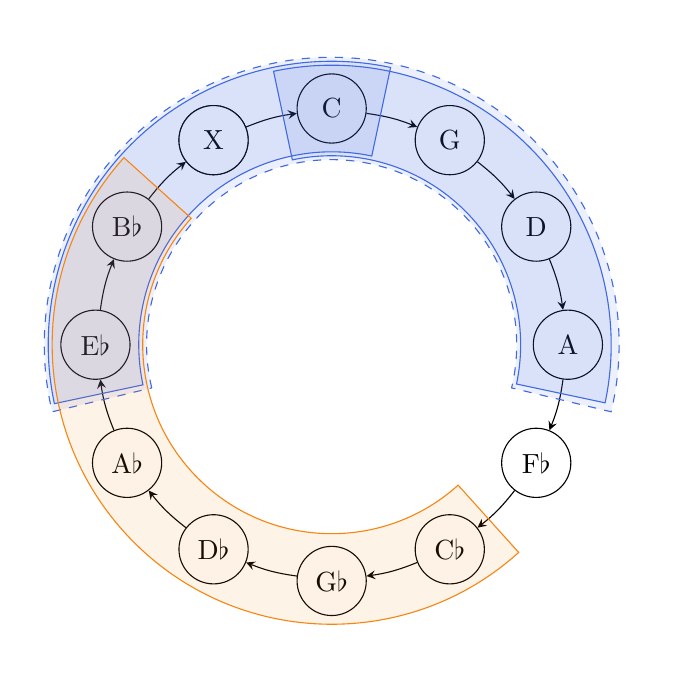
\begin{tikzpicture}[scale=1]
      % draw circle of fifths
      \circleoffifths{}
      % draw shading
      \arc{-3.45}{3.45}{\radius-0.65}{\radius+0.65}{RoyalBlue}{dashed}
      \arc{-3.4}{0.4}{\radius-0.55}{\radius+0.6}{RoyalBlue}{}
      \arc{-0.4}{3.4}{\radius-0.6}{\radius+0.55}{RoyalBlue}{}
      \arc{-1.6}{-7.4}{\radius-0.6}{\radius+0.55}{BurntOrange}{}
       \end{tikzpicture}
  } \\
  \scalebox{1}{
    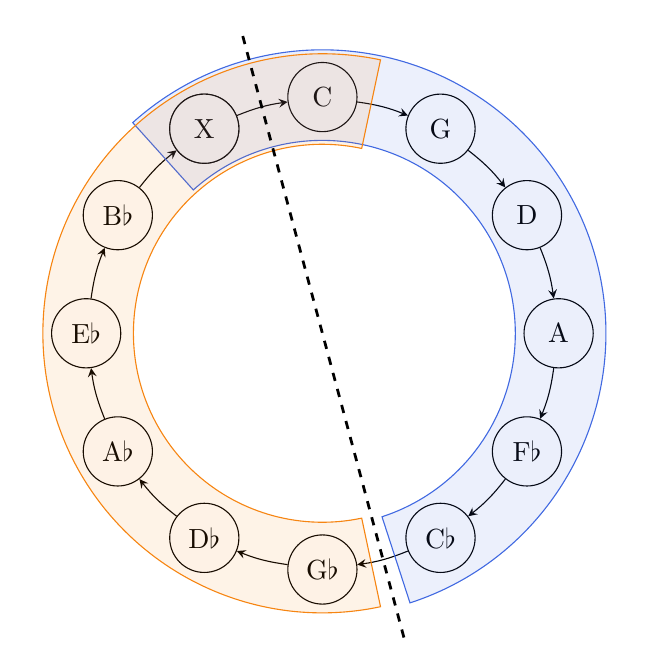
\begin{tikzpicture}[scale=1]
      % draw circle of fifths
      \circleoffifths{}
      % draw shading
      \arc{-1.4}{5.4}{\radius-0.55}{\radius+0.6}{RoyalBlue}{}
      \arc{0.4}{-6.4}{\radius-0.6}{\radius+0.55}{BurntOrange}{}
      \draw[line width=1pt,dashed] (-75:\radius+1) -- (105:\radius+1);
    \end{tikzpicture}
  }